\documentclass[11pt]{article}
\usepackage{amsgen,amsmath,amstext,amsbsy,amsopn,amssymb}
%\usepackage[dvips]{graphicx,color}
\usepackage{graphicx,color}
\usepackage{graphicx,color,bm}
\usepackage{epsfig}
\usepackage{enumerate}
\usepackage{float}

%\setlength{\oddsidemargin}{0.1 in} \setlength{\evensidemargin}{-0.1
%in} \setlength{\topmargin}{-0.6 in} \setlength{\textwidth}{6.5 in}
%\setlength{\textheight}{8.5 in} \setlength{\headsep}{0.75 in}
%\setlength{\parindent}{0 in} \setlength{\parskip}{0.1 in}

\textwidth 6.3in \textheight 8.8in \topmargin -0.5truein
\oddsidemargin .15truein
\parskip .1in
\renewcommand{\baselinestretch}{1.53}  % double spaced


\newcommand{\homework}[9]{
	\pagestyle{myheadings}
	\thispagestyle{plain}
	\newpage
	\setcounter{page}{1}
	\noindent
	\begin{center}
		\framebox{
			\vbox{\vspace{2mm}
				\hbox to 6.28in { {\bf Math531:~Regression - I  \hfill} }
				\vspace{6mm}
				\hbox to 6.28in { {\Large \hfill #1 (#2)  \hfill} }
				\vspace{6mm}
				\hbox to 6.28in { {\it Instructor: #3 \hfill} }
				\hbox to 6.28in { {\it Office hours: #4  \hfill #6}}
				\vspace{2mm}}
		}
	\end{center}
	\markboth{#1}{#1}
	\vspace*{4mm}
}

% ----------------------- MATH -------------------------
\def\av{\boldsymbol a}
\def\bv{\boldsymbol b}
\def\cv{\boldsymbol c}
\def\dv{\boldsymbol d}
\def\ev{\boldsymbol e}
\def\fv{\boldsymbol f}
\def\gv{\boldsymbol g}
\def\hv{\boldsymbol h}
\def\iv{\boldsymbol i}
\def\gv{\boldsymbol j}
\def\kv{\boldsymbol k}
\def\lv{\boldsymbol l}
\def\mv{\boldsymbol m}
\def\nv{\boldsymbol n}
\def\ov{\boldsymbol o}
\def\pv{\boldsymbol p}
\def\qv{\boldsymbol q}
\def\rv{\boldsymbol r}
\def\sv{\boldsymbol s}
\def\tv{\boldsymbol t}
\def\uv{\boldsymbol u}
\def\vv{\boldsymbol v}
\def\wv{\boldsymbol w}
\def\xv{\boldsymbol x}
\def\yv{\boldsymbol y}
\def\zv{\boldsymbol z}
\def\Av{\boldsymbol A}
\def\Bv{\boldsymbol B}
\def\Cv{\boldsymbol C}
\def\Dv{\boldsymbol D}
\def\Ev{\boldsymbol E}
\def\Fv{\boldsymbol F}
\def\Gv{\boldsymbol G}
\def\Hv{\boldsymbol H}
\def\Iv{\boldsymbol I}
\def\Gv{\boldsymbol J}
\def\Kv{\boldsymbol K}
\def\Lv{\boldsymbol L}
\def\Mv{\boldsymbol M}
\def\Nv{\boldsymbol N}
\def\Ov{\boldsymbol O}
\def\Pv{\boldsymbol P}
\def\Qv{\boldsymbol Q}
\def\Rv{\boldsymbol R}
\def\Sv{\boldsymbol S}
\def\Tv{\boldsymbol T}
\def\Uv{\boldsymbol U}
\def\Vv{\boldsymbol V}
\def\Wv{\boldsymbol W}
\def\Xv{\boldsymbol X}
\def\Yv{\boldsymbol Y}
\def\Zv{\boldsymbol Z}
\def\Abf{\mathbf A}
\def\Bbf{\mathbf B}
\def\Cbf{\mathbf C}
\def\Dbf{\mathbf D}
\def\Ebf{\mathbf E}
\def\Fbf{\mathbf F}
\def\Gbf{\mathbf G}
\def\Hbf{\mathbf H}
\def\Ibf{\mathbf I}
\def\Gbf{\mathbf J}
\def\Kbf{\mathbf K}
\def\Lbf{\mathbf L}
\def\Mbf{\mathbf M}
\def\Nbf{\mathbf N}
\def\Obf{\mathbf O}
\def\Pbf{\mathbf P}
\def\Qbf{\mathbf Q}
\def\Rbf{\mathbf R}
\def\Sbf{\mathbf S}
\def\Tbf{\mathbf T}
\def\Ubf{\mathbf U}
\def\Vbf{\mathbf V}
\def\Wbf{\mathbf W}
\def\Xbf{\mathbf X}
\def\Ybf{\mathbf Y}
\def\Jbf{\mathbf J}
\def\Zbf{\mathbf Z}
\def\Am{\mathrm A}
\def\Bm{\mathrm B}
\def\Cm{\mathrm C}
\def\Dm{\mathrm D}
\def\Em{\mathrm E}
\def\Fm{\mathrm F}
\def\Gm{\mathrm G}
\def\Hm{\mathrm H}
\def\Im{\mathrm I}
\def\Gm{\mathrm J}
\def\Km{\mathrm K}
\def\Lm{\mathrm L}
\def\Mm{\mathrm M}
\def\Nm{\mathrm N}
\def\Om{\mathrm O}
\def\Pm{\mathrm P}
\def\Qm{\mathrm Q}
\def\Rm{\mathrm R}
\def\Sm{\mathrm S}
\def\Tm{\mathrm T}
\def\Um{\mathrm U}
\def\mv{\mathrm V}
\def\Wm{\mathrm W}
\def\Xm{\mathrm X}
\def\Ym{\mathrm Y}
\def\Zm{\mathrm Z}
\newcommand{\Ac}{\mathcal{A}}
\newcommand{\Bc}{\mathcal{B}}
\newcommand{\Cc}{\mathcal{C}}
\newcommand{\Dc}{\mathcal{D}}
\newcommand{\Ec}{\mathcal{E}}
\newcommand{\Fc}{\mathcal{F}}
\newcommand{\Gc}{\mathcal{G}}
\newcommand{\Hc}{\mathcal{H}}
\newcommand{\Ic}{\mathcal{I}}
\newcommand{\Jc}{\mathcal{J}}
\newcommand{\Kc}{\mathcal{K}}
\newcommand{\Lc}{\mathcal{L}}
\newcommand{\Mc}{\mathcal{M}}
\newcommand{\Nc}{\mathcal{N}}
\newcommand{\Oc}{\mathcal{O}}
\newcommand{\Pc}{\mathcal{P}}
\newcommand{\Qc}{\mathcal{Q}}
\newcommand{\Rc}{\mathcal{R}}
\newcommand{\Sc}{\mathcal{S}}
\newcommand{\Tc}{\mathcal{T}}
\newcommand{\Uc}{\mathcal{U}}
\newcommand{\Vc}{\mathcal{V}}
\newcommand{\Wc}{\mathcal{W}}
\newcommand{\Xc}{\mathcal{X}}
\newcommand{\Yc}{\mathcal{Y}}
\newcommand{\Zc}{\mathcal{Z}}
\newcommand{\alphav}{\mbox{\boldmath{$\alpha$}}}
\newcommand{\betav}{\mbox{\boldmath{$\beta$}}}
\newcommand{\gammav}{\mbox{\boldmath{$\gamma$}}}
\newcommand{\deltav}{\mbox{\boldmath{$\delta$}}}
\newcommand{\epsilonv}{\mbox{\boldmath{$\epsilon$}}}
\newcommand{\zetav}{\mbox{\boldmath$\zeta$}}
\newcommand{\etav}{\mbox{\boldmath{$\eta$}}}
\newcommand{\iotav}{\mbox{\boldmath{$\iota$}}}
\newcommand{\kappav}{\mbox{\boldmath{$\kappa$}}}
\newcommand{\lambdav}{\mbox{\boldmath{$\lambda$}}}
\newcommand{\muv}{\mbox{\boldmath{$\mu$}}}
\newcommand{\nuv}{\mbox{\boldmath{$\nu$}}}
\newcommand{\xiv}{\mbox{\boldmath{$\xi$}}}
\newcommand{\omicronv}{\mbox{\boldmath{$\omicron$}}}
\newcommand{\piv}{\mbox{\boldmath{$\pi$}}}
\newcommand{\rhov}{\mbox{\boldmath{$\rho$}}}
\newcommand{\sigmav}{\mbox{\boldmath{$\sigma$}}}
\newcommand{\tauv}{\mbox{\boldmath{$\tau$}}}
\newcommand{\upsilonv}{\mbox{\boldmath{$\upsilon$}}}
\newcommand{\phiv}{\mbox{\boldmath{$\phi$}}}
\newcommand{\varphiv}{\mbox{\boldmath{$\varphi$}}}
\newcommand{\chiv}{\mbox{\boldmath{$\chi$}}}
\newcommand{\psiv}{\mbox{\boldmath{$\psi$}}}
\newcommand{\omegav}{\mbox{\boldmath{$\omega$}}}
\newcommand{\Sigmav}{\mbox{\boldmath{$\Sigma$}}}
\newcommand{\Lambdav}{\mbox{\boldmath{$\Lambda$}}}
\newcommand{\Deltav}{\mbox{\boldmath{$\Delta$}}}
\newcommand{\Omegav}{\mbox{\boldmath{$\Omega$}}}
\newcommand{\varepsilonv}{\mbox{\boldmath{$\varepsilon$}}}

\newcommand{\eps}{\varepsilon}
\newcommand{\epsv}{\mbox{\boldmath{$\varepsilon$}}}

\def\1v{\mathbf 1}
\def\0v{\mathbf 0}
\def\Id{\mathbf I} % identity matrix
\newcommand{\ind}[1]{\mathbbm{1}_{\left[ {#1} \right] }}
\newcommand{\Ind}[1]{\mathbbm{1}_{\left\{ {#1} \right\} }}
\newcommand\indep{\protect\mathpalette{\protect\independenT}{\perp}}\def\independenT#1#2{\mathrel{\rlap{$#1#2$}\mkern2mu{#1#2}}}
\newcommand{\QED}{\begin{flushright} {\bf QED} \end{flushright}}
\newcommand{\R}{\mathbb R}
\newcommand{\Real}{\mathbb R}
\newcommand{\C}{\mathbb C}
\newcommand{\E}{\mathbb E}
\newcommand{\sgn}{\mathop{\mathrm{sign}}}
\def\Pr{\mathrm P}
\def\pr{\mathrm P}
\newcommand{\Var}{\mathop{\rm Var}}
\newcommand{\var}{\mathop{\rm Var}}
\newcommand{\Cov}{\mathop{\rm Cov}}
\newcommand{\cov}{\mathop{\rm Cov}}
\newcommand{\Corr}{\mathop{\rm Corr}}
\newcommand{\ang}{\mathop{\rm Angle}}
\newcommand{\tr}{\mathop{\rm trace}}
\newcommand{\proj}{\mathop{\rm Proj}}
\newcommand{\rank}{\mathop{\rm rank}}

\newcommand{\diag}{\mathop{\rm diag}}
\newcommand{\Diag}{\mathop{\rm diag}}
\newcommand{\sk}{\vspace{0.5cm}}
\newcommand{\ds}{\displaystyle}
\newcommand{\mb}{\mbox}
\newcommand{\wh}{\widehat}
\newcommand{\argmin}{\operatornamewithlimits{argmin}}
\newcommand{\argmax}{\operatornamewithlimits{argmax}}

\newcommand{\norm}[1]{\|#1\|}
\newcommand{\abs}[1]{\left\vert#1\right\vert}
\newcommand{\set}[1]{\left\{#1\right\}}

\newcommand{\To}{\longrightarrow}

\def\equalLaw{\stackrel{\mathcal{L}}{=}}
\def\equallaw{\stackrel{\mathcal{L}}{=}}

\def\half{\frac{1}{2}}

\usepackage{caption}

\begin{document}

\begin{title}
	{\Large\bf Homework 5, DATA 556: Due Tuesday, 10/31/2018}
\end{title}

\author{\bf Alexander Van Roijen}

\maketitle

\newpage
Please complete the following:
\begin{enumerate}
\item Problem 1
Let $U \sim $Unif(a, b).
\begin{enumerate}
	\item Use simulations in R (the statistical programming language) to numerically estimate the median and
	the mode of U for a = 0 and b = 2.
	\begin{verbatim}
	> binUnif= function(n,a,b)
	+ {
	+   resultsog = runif(n,a,b)
	+   results = floor(resultsog*10)
	+   data = data.frame(results)
	+   vals = seq(a,b,.1)
	+   p<-ggplot(data=data, aes(x=factor(data[,1]))) +geom_bar(stat="count") + scale_x_discrete(labels=vals)
	+   p
	+   #barplot(results,main="whatev",width=0.5)
	+   print(median(resultsog))
	+   getmode = table(resultsog)
	+   print(which.max(getmode))
	+   #print(forMode[c(1:10),])
	+ }
	> #this is 1a
	> set.seed(123)
	> n=1000000
	> binUnif(n,0,2)
	[1] 0.9983065
	0.0349205480888486 
	17519 
	\end{verbatim}
	\begin{figure}[H]
		\centering
		\caption{Mode roughly equivalent across all values of x}
		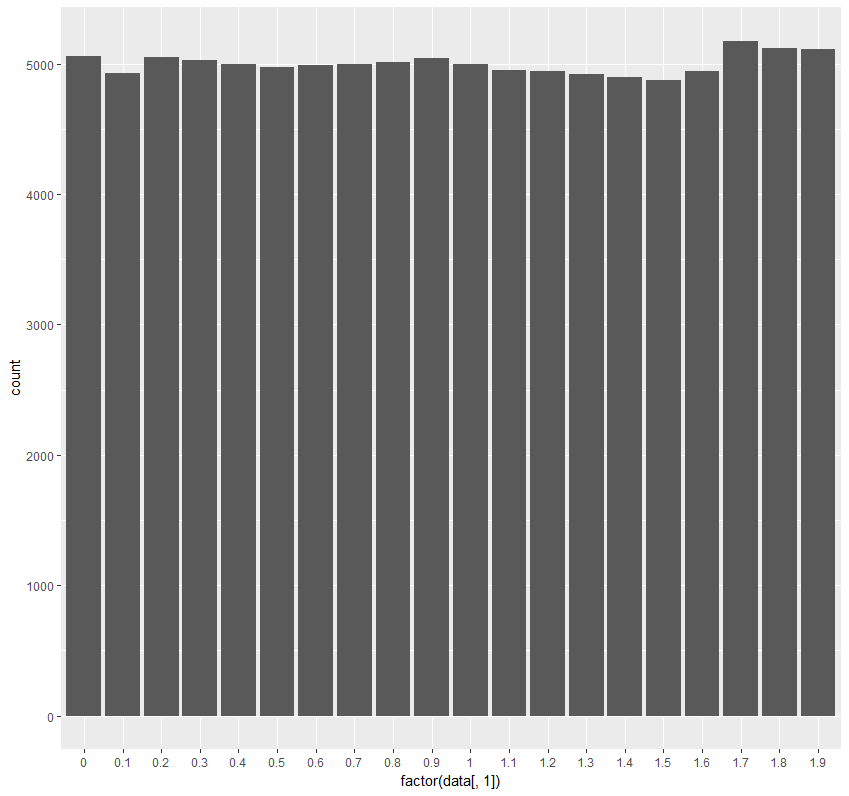
\includegraphics[scale=.6]{Rplot.png}
	\end{figure}
	\item Find the Median and Mode of $U \sim $ Unif(a,b)
	\begin{gather}
	\text{Take the result form above and take the derivative }\\
	f(X|X>a) = F'(X|X>a) = \frac{dF(X|X>a)}{dx} = \frac{F'(x)-F'(a)}{1-F(a)} \text{ with} \frac{dF(a)}{dx} = 0 \\
	=> f(X|X>a) =\frac{f(x)}{1-F(a)}
	\end{gather}
\end{enumerate}
\item Let $ X \sim  $ Expo($ \lambda $)
\\
\begin{enumerate}
	\item Use R to simulate median and mode of Expo(2)
	\\
	\begin{verbatim}
	expoMedMode = function(n,rate)
	+ {
	+   resultsog = rexp(n,rate=rate)
	+   results = floor(resultsog*10)
	+   data = data.frame(results)
	+   data = data.frame(data[data[,1]<25,])
	+   vals = seq(0,2.5,.1)
	+   p<-ggplot(data=data, aes(x=factor(data[,1]))) +geom_bar(stat="count") + scale_x_discrete(labels=vals)
	+   print(p)
	+   #barplot(results,main="whatev",width=0.5)
	+   print(median(resultsog))
	+   getmode = table(resultsog)
	+   print(which.max(getmode))
	+ }
	> #this is 2a
	> set.seed(123)
	> n=1000000
	> expoMedMode(n,2)
	[1] 0.3467215
	0.00334986066445708 
	6662 
	\end{verbatim}
	\begin{figure}[H]
		\centering
		\caption{Mode of an exponential with rate of 2 around 0 and median around .3467}
		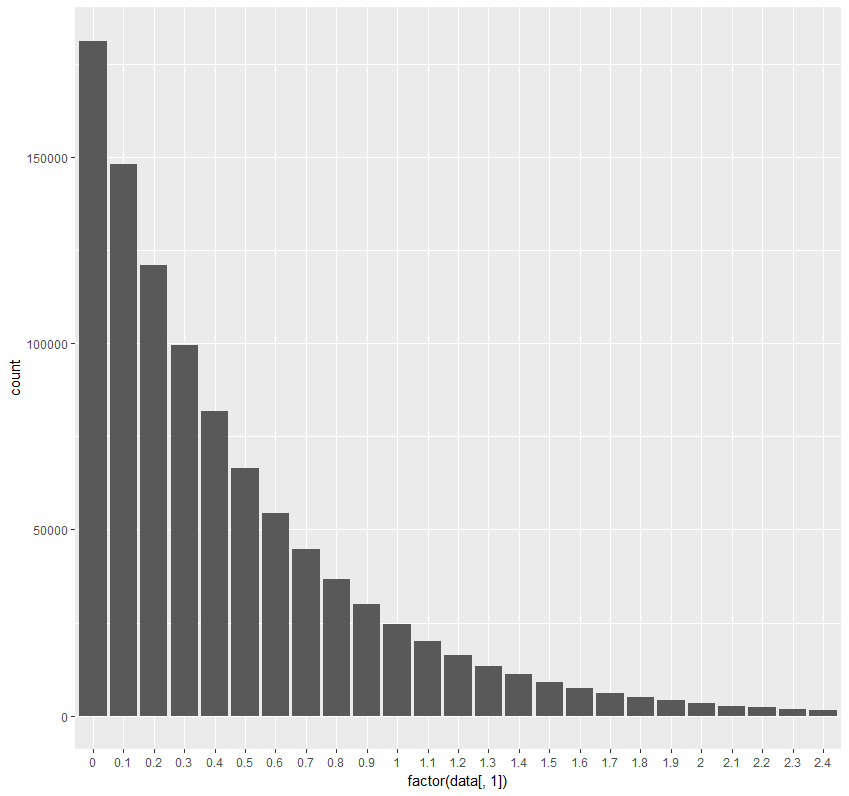
\includegraphics[scale=.6]{barplotexpo.png}
	\end{figure}
	This overall makes sense, as we will show below, 0 is the mode of the exponential distribution. This is confirmed as well by the barplot shown above.
	\item Find the Median and Mode of $X \sim $ Expo($\lambda $)
\end{enumerate}
\item Let X be Discrete Uniform on 1,2,3,4,5...n .
\begin{enumerate}
	\item  Use simulations in R to numerically estimate all medians and all modes of X for n = 1,2,3...10.
	\begin{verbatim}
	> #this is 3a
	> set.seed(433)
	> counter = 1
	> n=10
	> size = 1000
	> while(counter <= n)
	+ {
	+   binUnif(size,1,counter,1,1)
	+   counter = counter + 1
	+ }
	[1] "From 1 to 1"
	[1] 1
	1 
	1 
	[1] "From 1 to 2"
	[1] 1.505739
	1.0011387350969 
	1 
	[1] "From 1 to 3"
	[1] 2.025223
	1.00209179287776 
	1 
	[1] "From 1 to 4"
	[1] 2.502714
	1.00117637915537 
	1 
	[1] "From 1 to 5"
	[1] 2.957827
	1.00255306344479 
	1 
	[1] "From 1 to 6"
	[1] 3.368198
	1.00341863720678 
	1 
	[1] "From 1 to 7"
	[1] 4.004081
	1.0143808578141 
	1 
	[1] "From 1 to 8"
	[1] 4.470458
	1.00075664301403 
	1 
	[1] "From 1 to 9"
	[1] 5.058819
	1.0038467105478 
	1 
	[1] "From 1 to 10"
	[1] 5.422321
	1.01815693522803 
	1 
	\end{verbatim}
	\begin{figure}[H]
		\centering
		\caption{Mode across demonstrated from Unif(1,1)}
		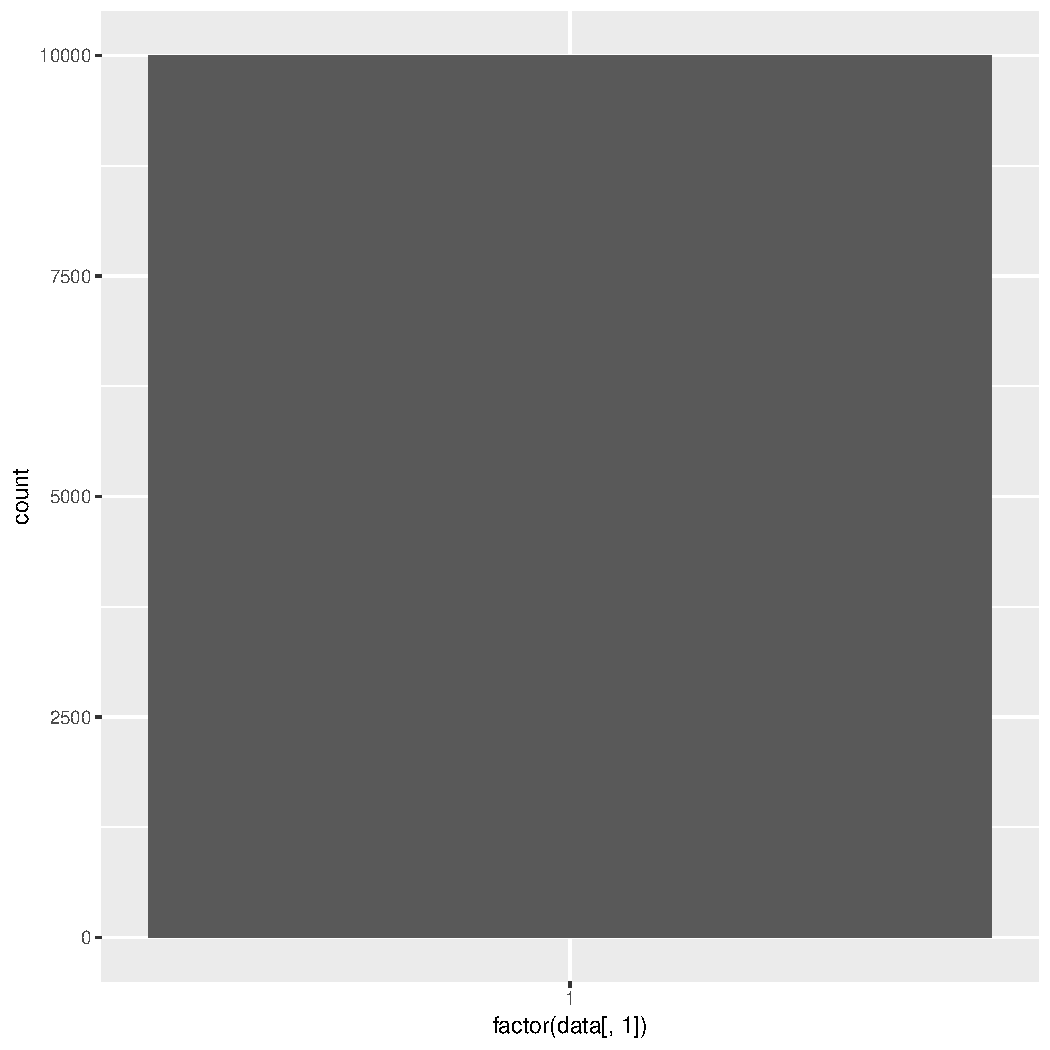
\includegraphics[scale=.4]{1graph.pdf}
	\end{figure}
	\begin{figure}[H]
		\centering
		\caption{Mode across demonstrated from Unif(1,1)}
		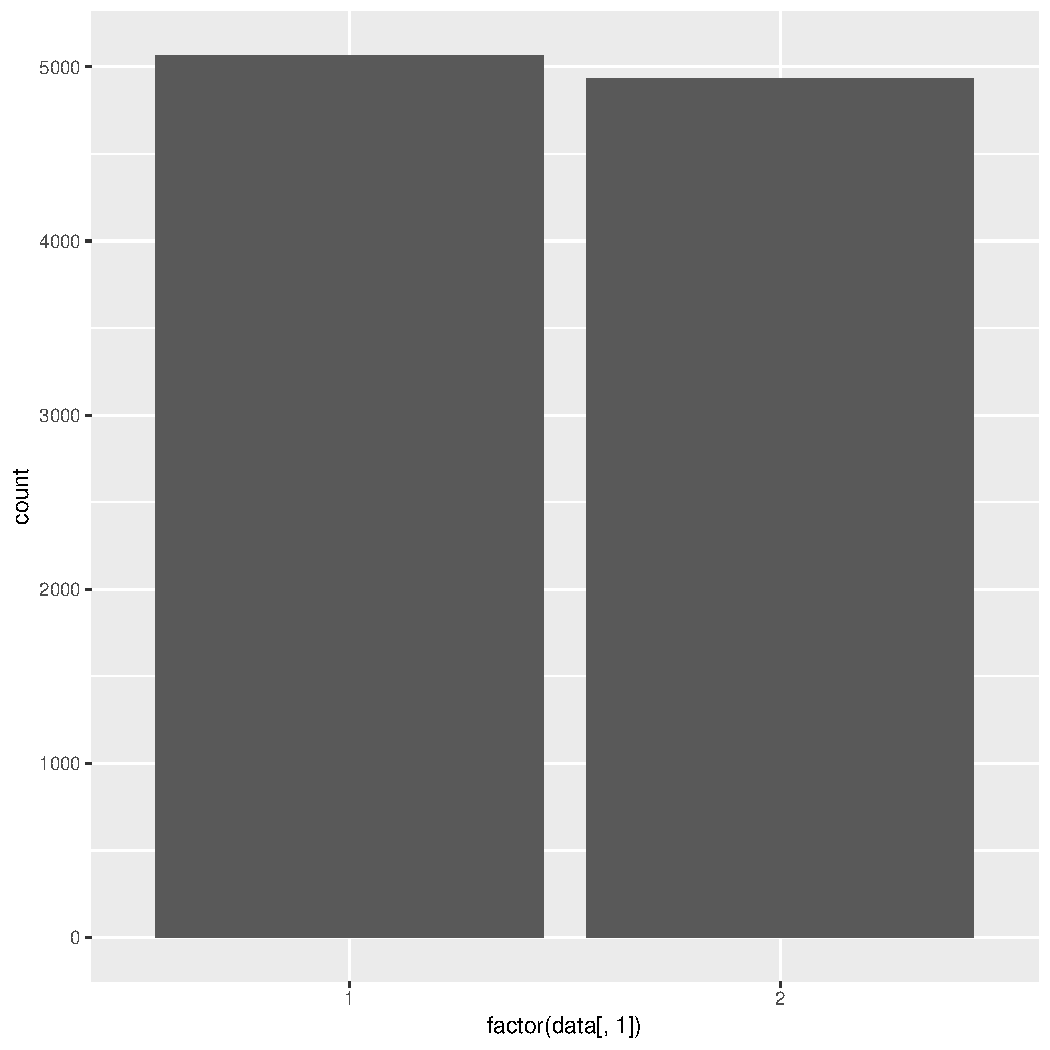
\includegraphics[scale=.4]{2graph.pdf}
	\end{figure}
	\begin{figure}[H]
		\centering
		\caption{Mode across demonstrated from Unif(1,1)}
		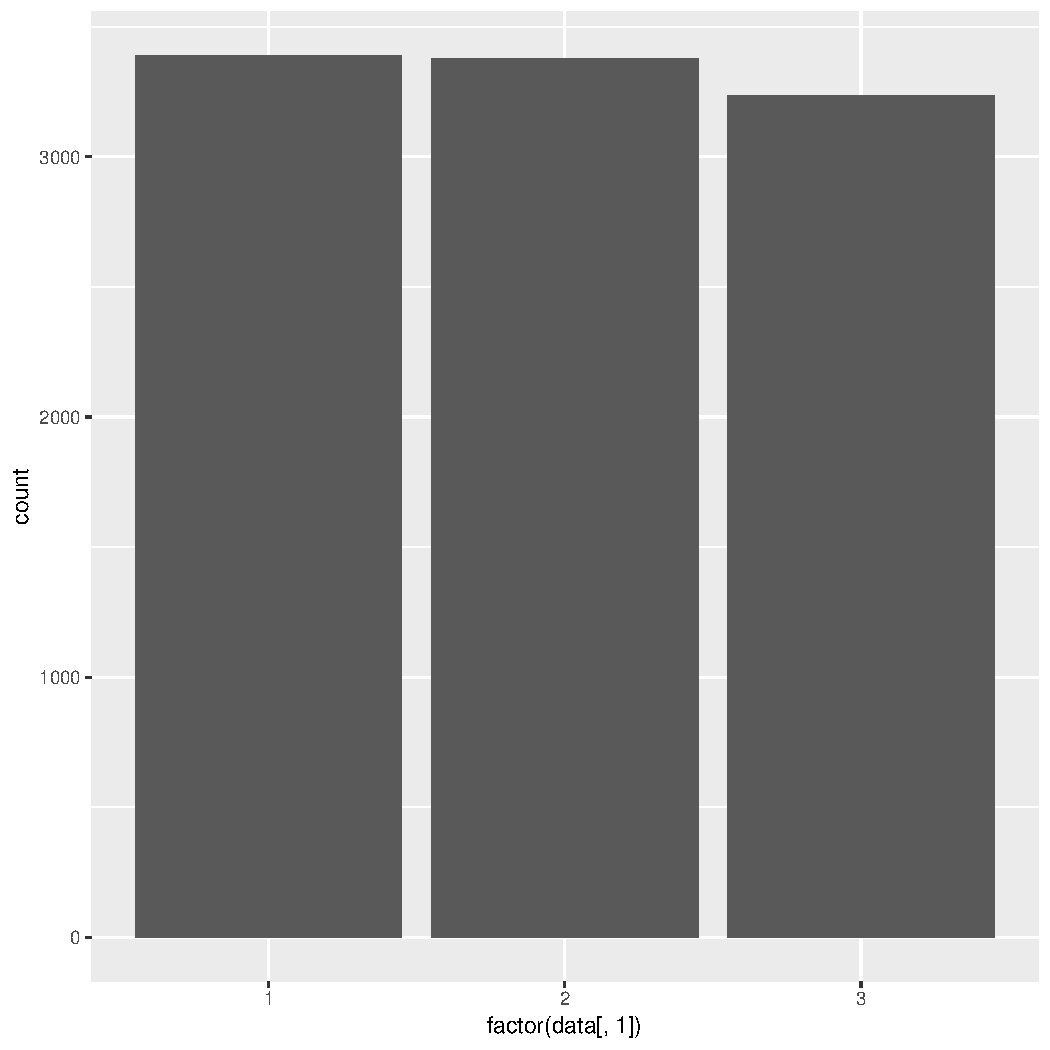
\includegraphics[scale=.4]{3graph.pdf}
	\end{figure}
	\begin{figure}[H]
		\centering
		\caption{Mode across demonstrated from Unif(1,1)}
		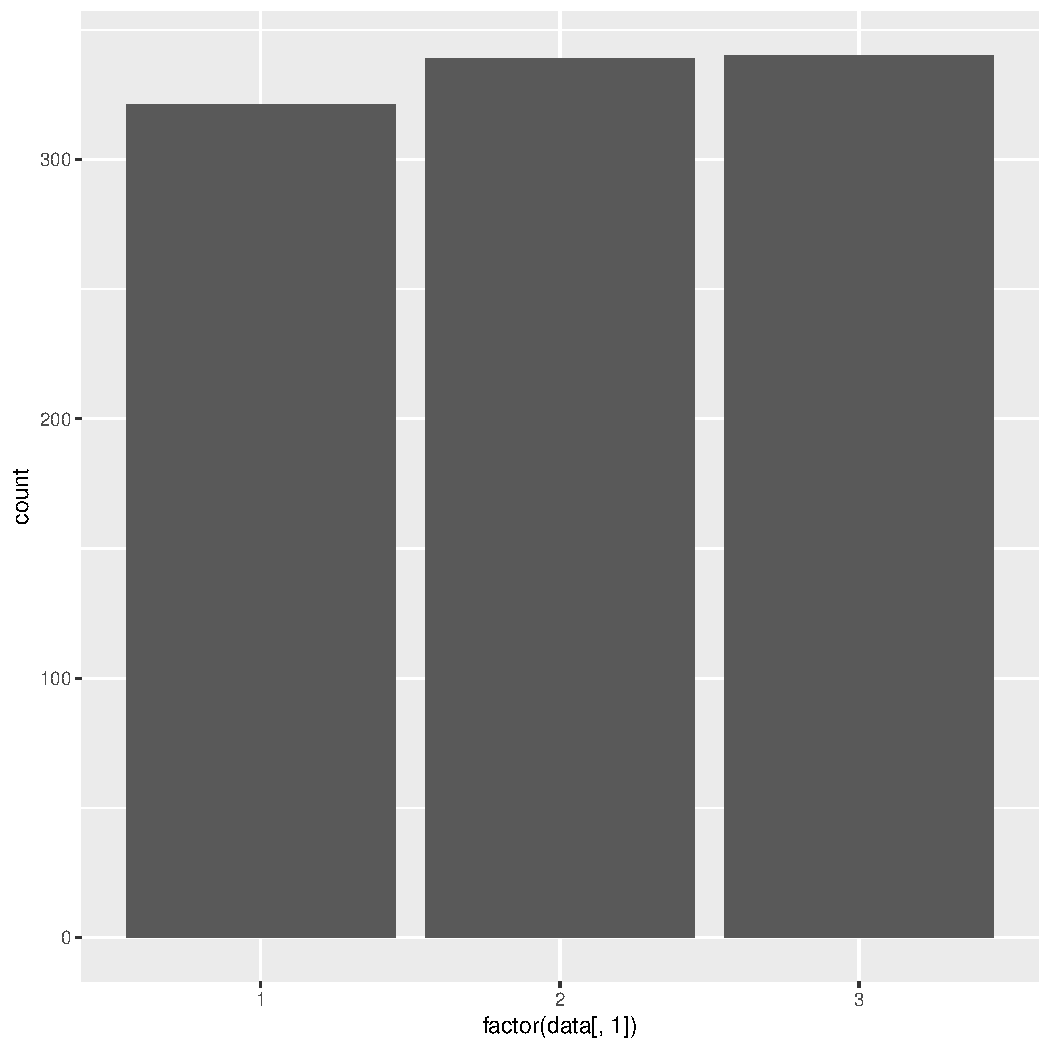
\includegraphics[scale=.4]{4graph.pdf}
	\end{figure}
	\begin{figure}[H]
		\centering
		\caption{Mode across demonstrated from Unif(1,1)}
		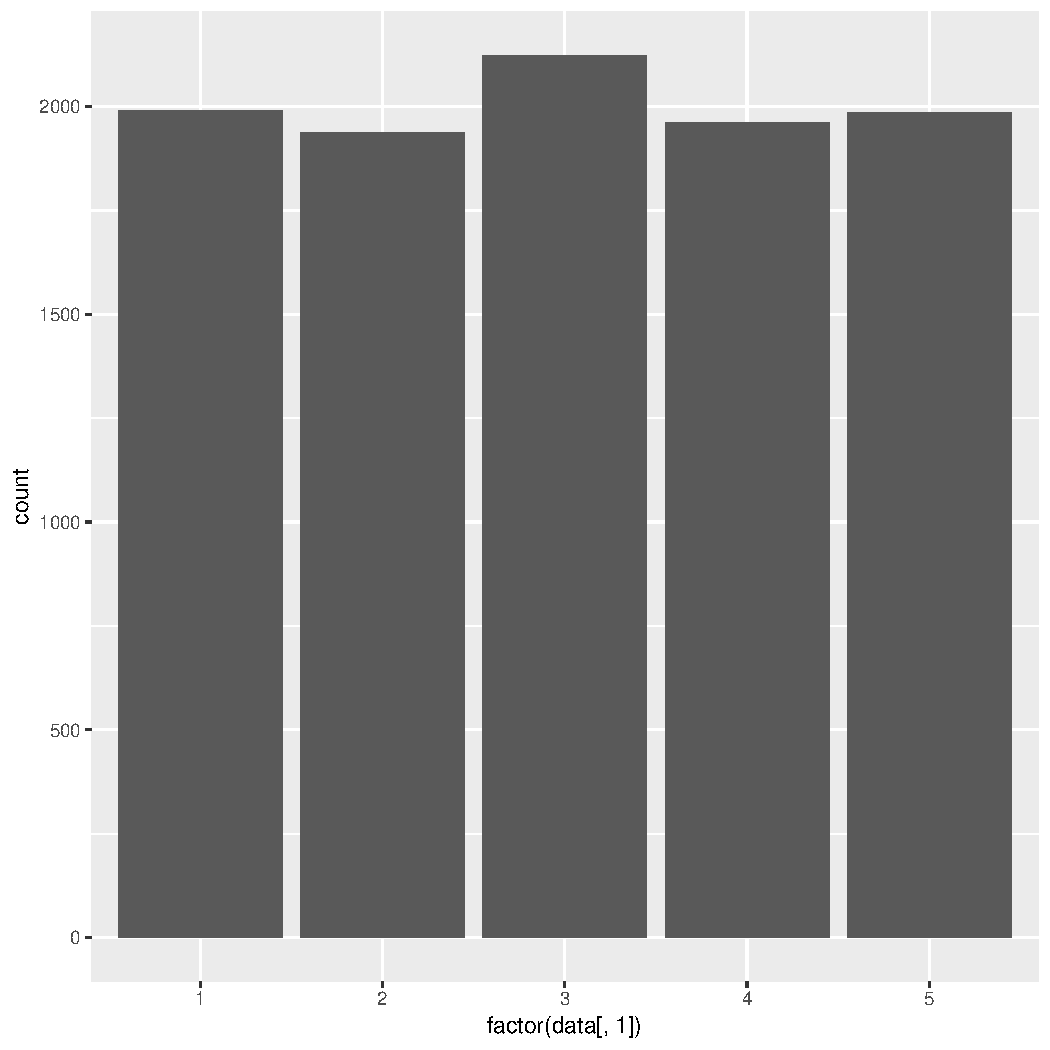
\includegraphics[scale=.4]{5graph.pdf}
	\end{figure}
	\begin{figure}[H]
		\centering
		\caption{Mode across demonstrated from Unif(1,1)}
		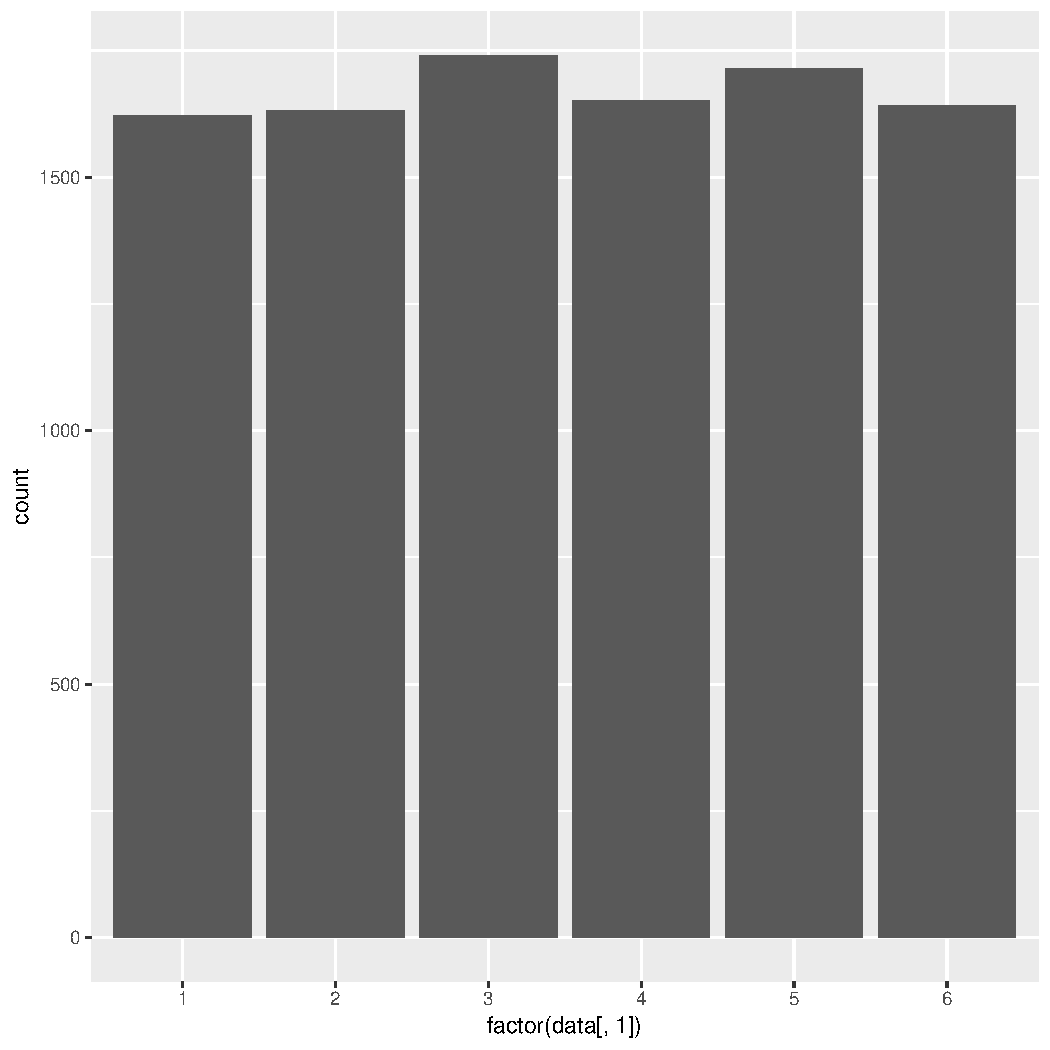
\includegraphics[scale=.4]{6graph.pdf}
	\end{figure}
	\begin{figure}[H]
		\centering
		\caption{Mode across demonstrated from Unif(1,1)}
		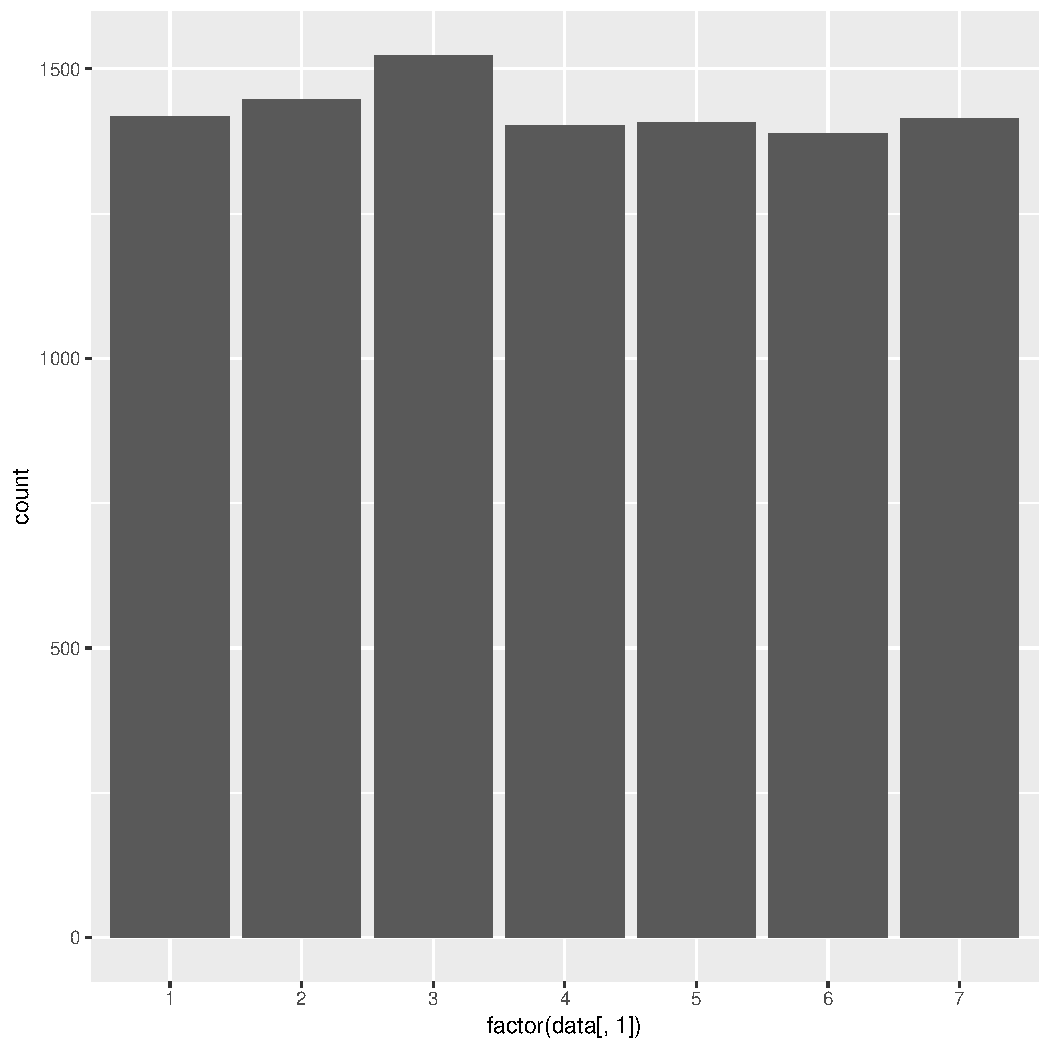
\includegraphics[scale=.4]{7graph.pdf}
	\end{figure}
	\begin{figure}[H]
		\centering
		\caption{Mode across demonstrated from Unif(1,1)}
		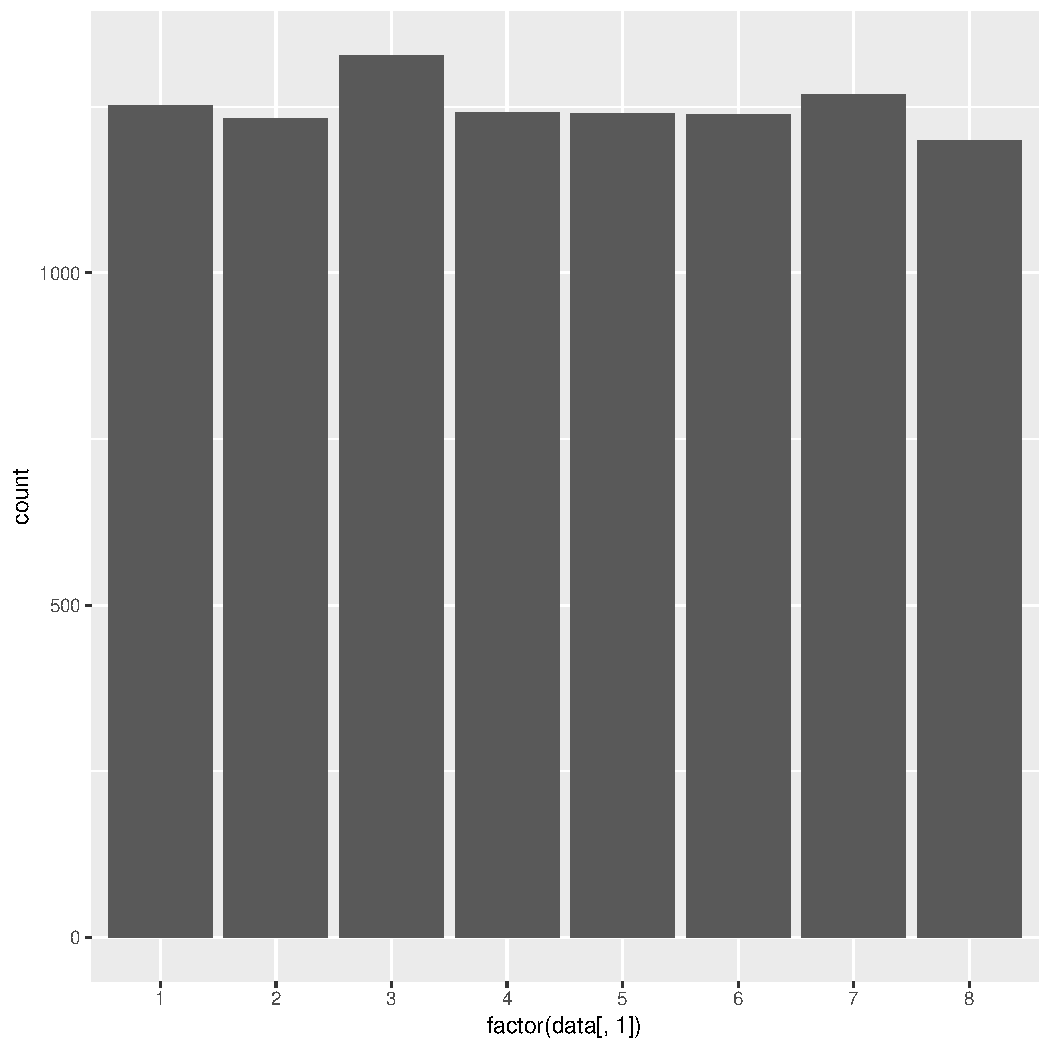
\includegraphics[scale=.4]{8graph.pdf}
	\end{figure}
	\begin{figure}[H]
		\centering
		\caption{Mode across demonstrated from Unif(1,1)}
		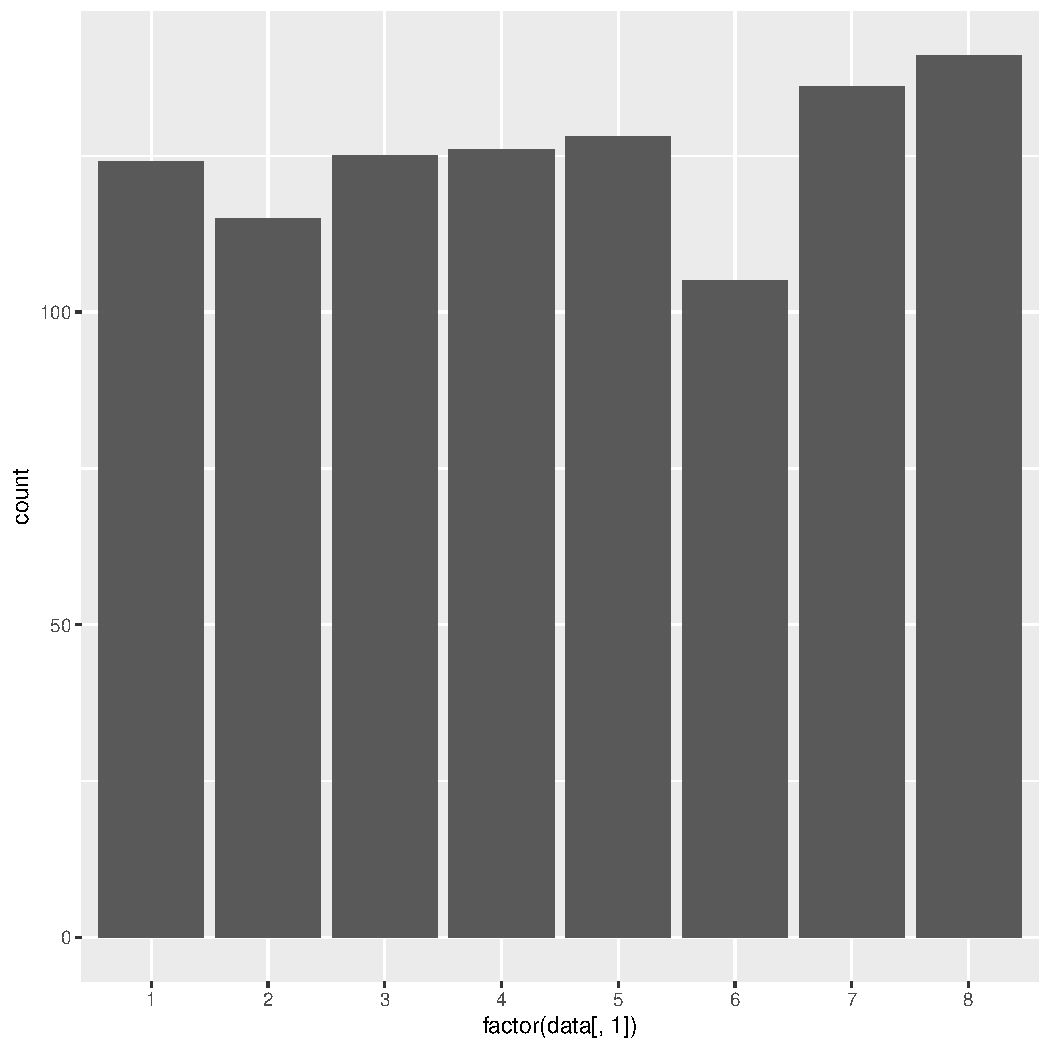
\includegraphics[scale=.4]{9graph.pdf}
	\end{figure}
	\begin{figure}[H]
		\centering
		\caption{Mode across demonstrated from Unif(1,1)}
		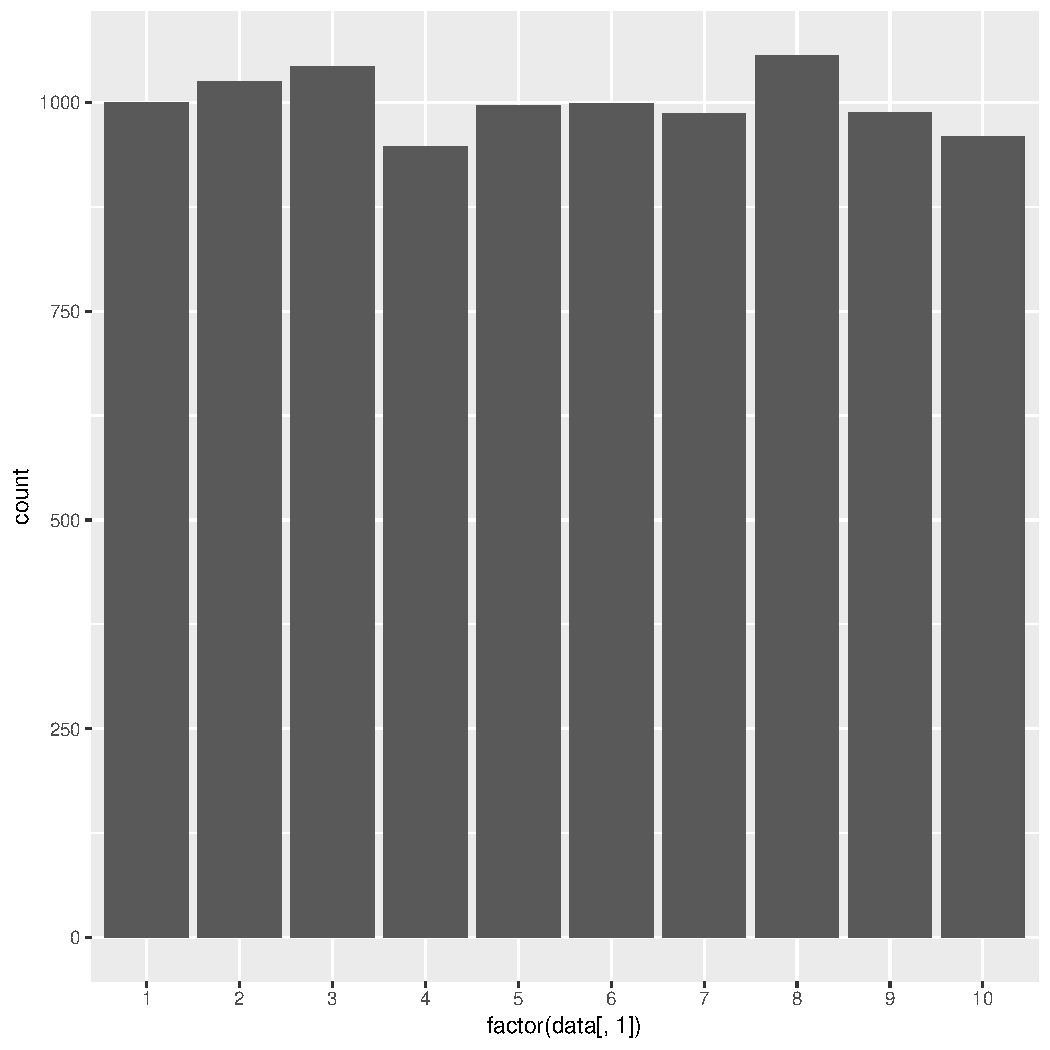
\includegraphics[scale=.4]{10graph.pdf}
	\end{figure}
	
	\item Find All medians and modes of X\\
	Note the mode is trivial, as it is a similar case to 1.
	\begin{gather}
	\text{Want } P(X=c)\ge P(X=x)\forall x \in 1,2,...n\\
	=> \frac{1}{n-1+1} \ge \frac{1}{n-1+1}  \text{ by def of discrete Uniform}\\
	=> c=x \forall x \in 1,2,3,...n \text{ which is almost the same as 1}\\
	\text{Notable difference is that in the discrete case, c can only take discrete values}\\
	\text{Now the median}\\
	\text{Want } P(X\le x) \ge \frac{1}{2} \& P(X\ge x) \ge \frac{1}{2}\\
	P(X\le x) = \sum_{i=1}^{x}\frac{1}{n} = \frac{x}{n} \ge \frac{1}{2} => x \ge \frac{n}{2}\\
	\text{However, we can observe the patterns noted in the graphs below}\\
	\text{If n is odd, the previous conclusion is the only solution as }\\
	\text{if you go above or below } \frac{n}{2} \text{ you lose the probability @ } x = \frac{n}{2}\\
	\text{This is true as we have a jump exactly at }\frac{n}{2}\\
	\text{In the case n is even, you have some wiggle room}\\
	\text{There is no jump at }\frac{n}{2}\\
	\text{In fact, the next jump is at }\frac{n}{2}+1\\
	\text{This means we have medians from }[\frac{n}{2},\frac{n}{2}+1]\\
	\text{One last important factor to note, is that this result relies heavily on}\\
	\text{how we define the median and our environment}\\
	\text{In general we have}\\
	 Median(X) = 
	 \begin{cases}
	 \frac{n}{2} & n=\text{odd} \\
	 [\frac{n}{2},\frac{n}{2}+1] & n=\text{even}
	 \end{cases}
	\end{gather}
	\begin{figure}[H]
		\centering
		\caption{(n=5)Note the jumps taking place on the discrete values}
		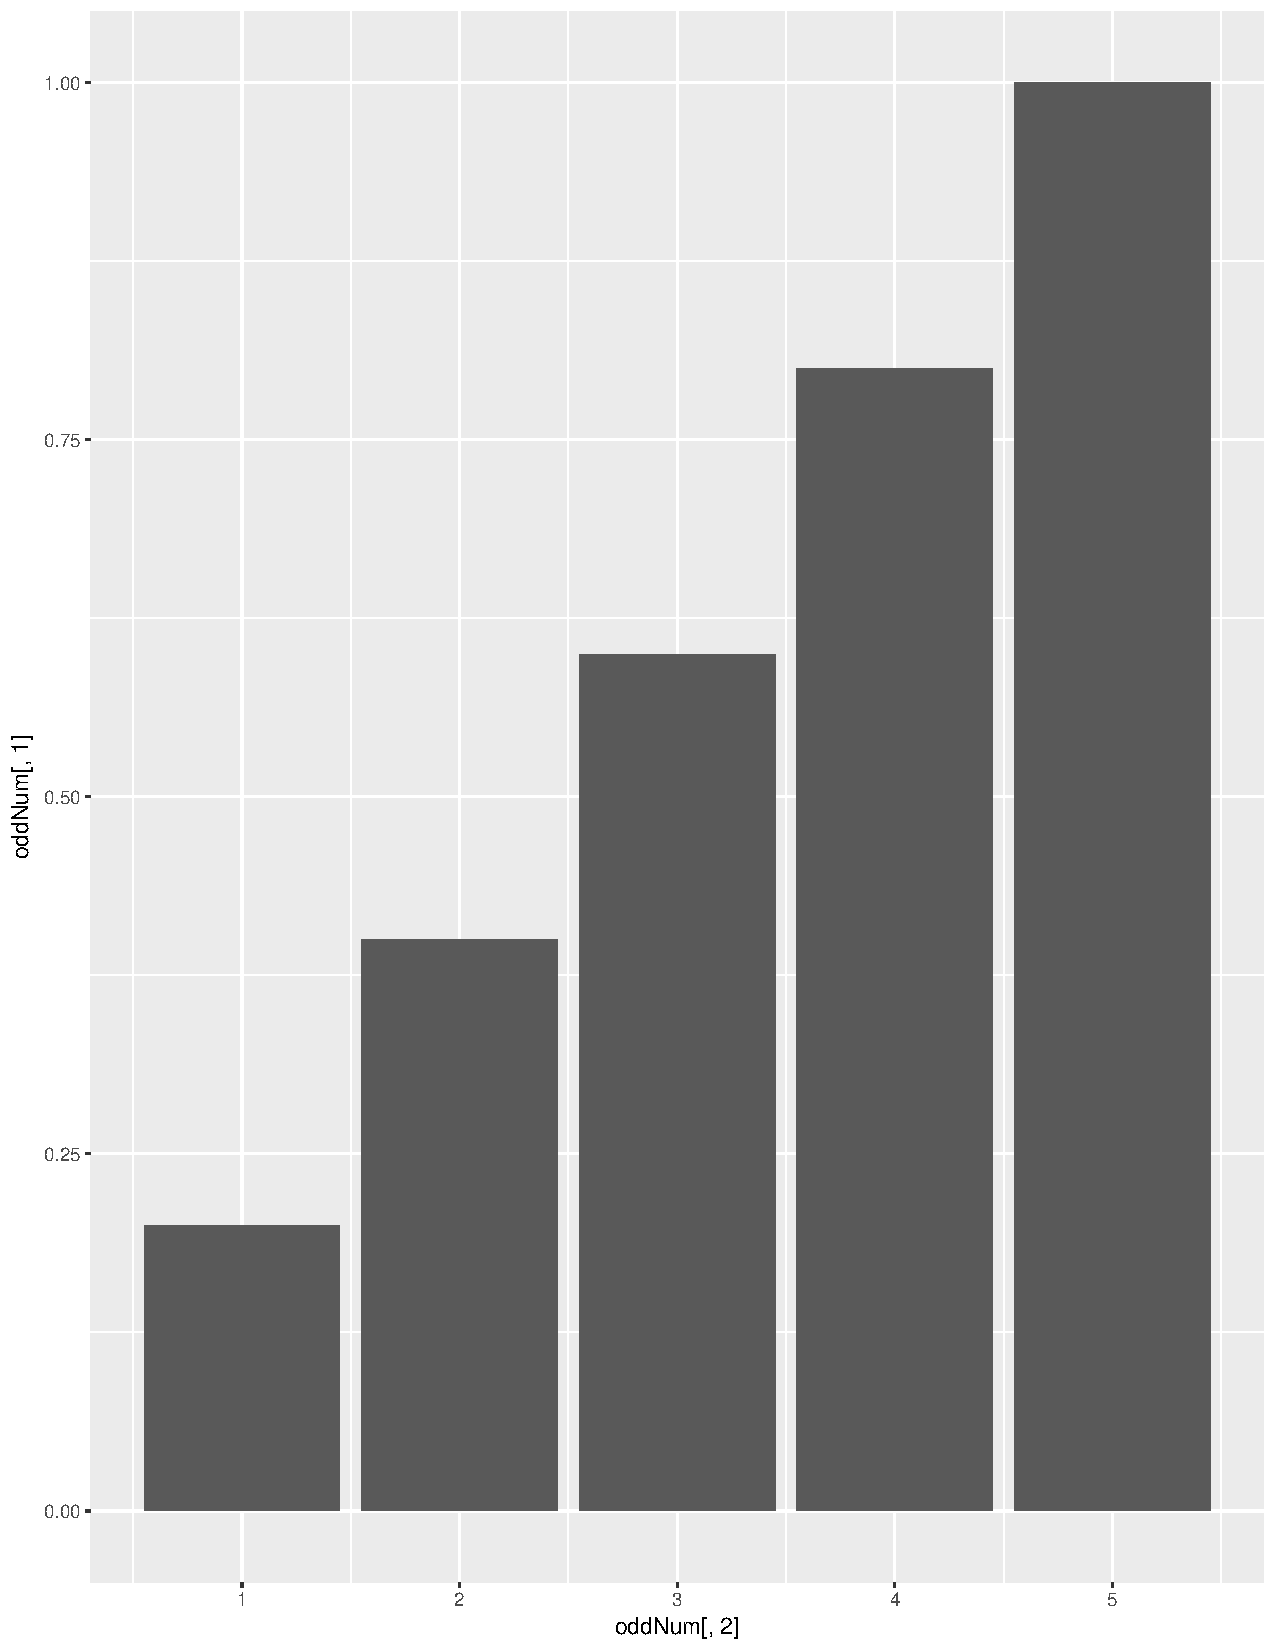
\includegraphics[scale=.4]{discreteOdd.pdf}
	\end{figure}
	\begin{figure}[H]
		\centering
		\caption{(n=6)These jump patterns hold for all discrete n}
		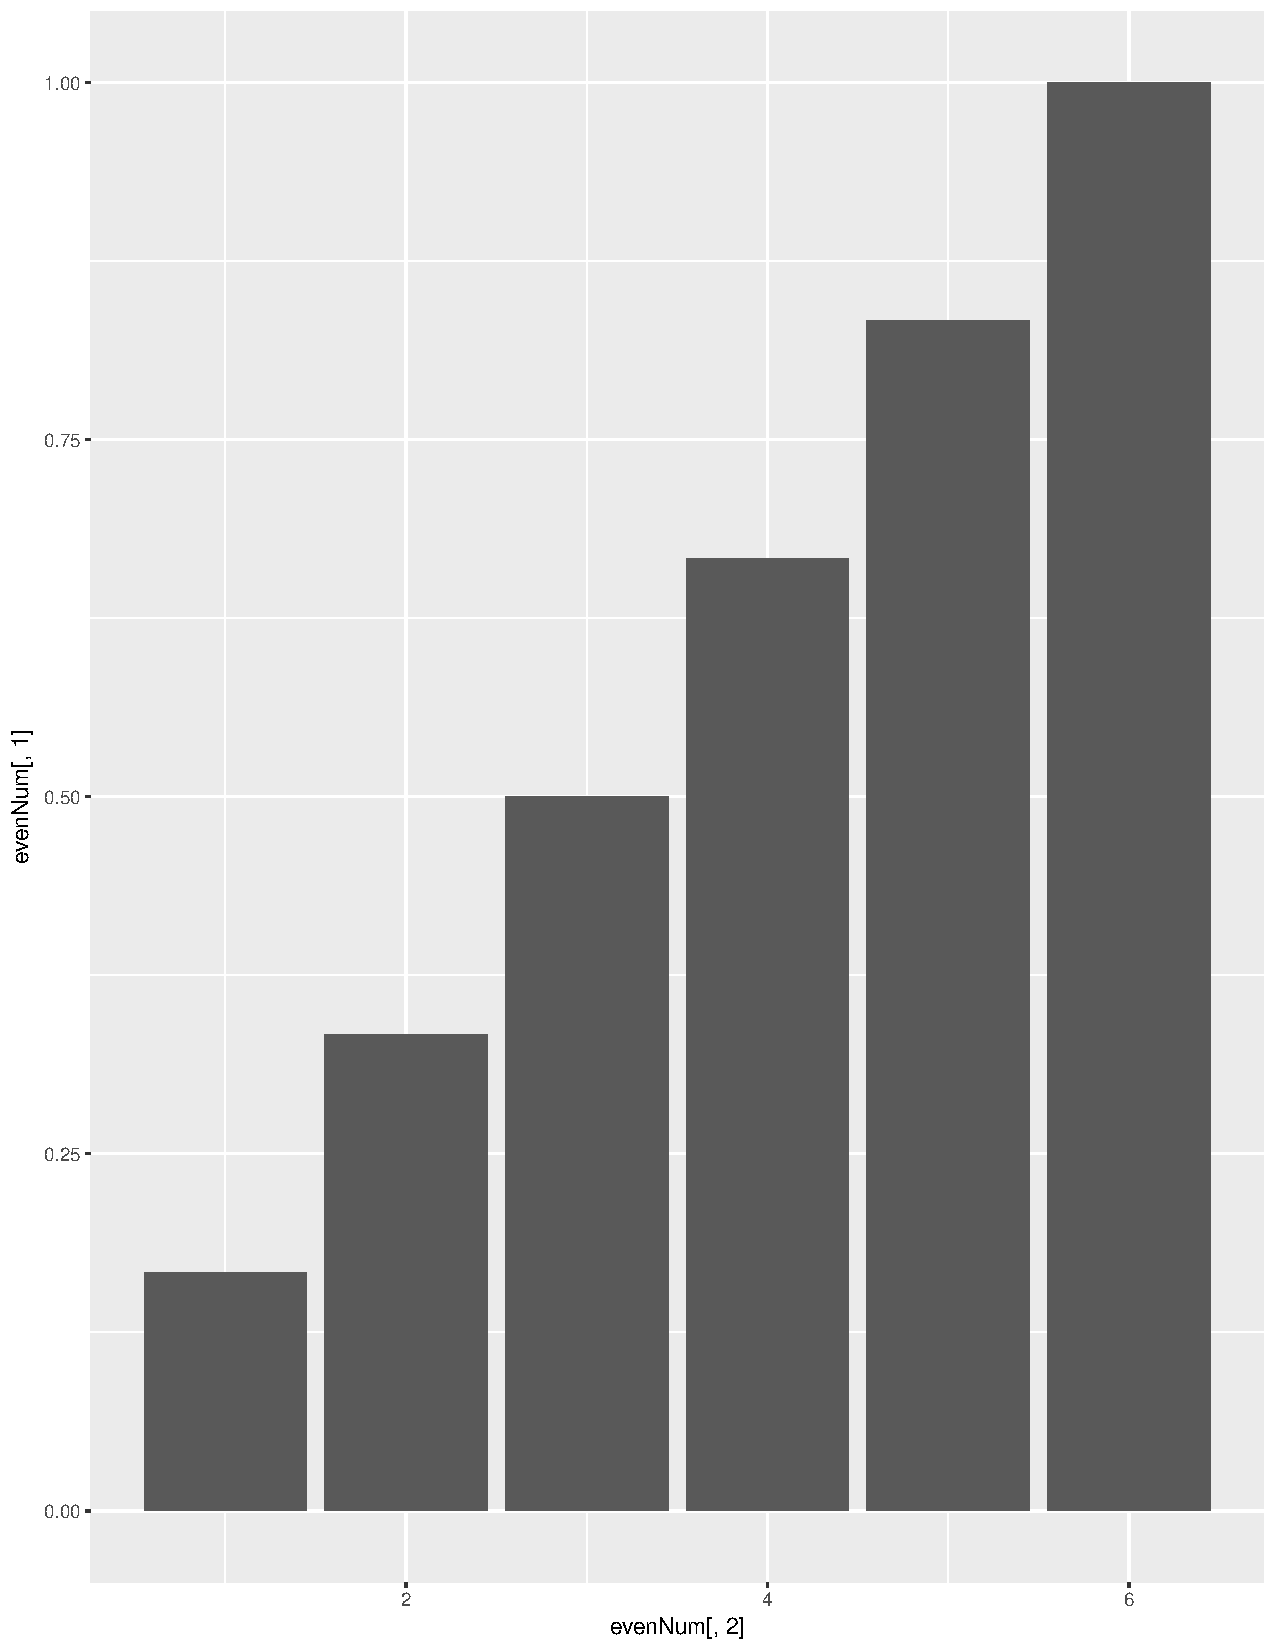
\includegraphics[scale=.4]{evenDisc.pdf}
	\end{figure}
\end{enumerate}
\item Let $U_1,...,U_n$ be i.i.d. $Unif(0,1)$, and $X = max(U_1,...,U_n)$.
\begin{enumerate}
	\item What is the PDF of X?
	\begin{gather}
		\text{CDF} = P(X \le x) = P(U_1 \le x , ... , U_n \le x) = P(U_1 \le x) *  ... * P(U_n \le x) \text{ since i.i.d}\\
		=> \text{CDF} = x*x*x...*x = x^n => \text{ PDF } = \frac{dF}{dx} = n*x^{n-1} \text{ with } 0 \le x \le 1
	\end{gather}
	\item what is the $E[X]$
	\begin{gather}
		\int_{-\infty}^{\infty}x*f(x) = \int_{0}^{1}x*f(x) = \int_{0}^{1}x*n*x^{n-1} = \int_{0}^{1}n*x^{n} =\frac{n}{n+1}*(1^n) - 0 = \frac{n}{n+1}
	\end{gather}
	\item R simulation results / approx
	\begin{verbatim}
		> #4c
		> set.seed(123)
		> n=10
		> runplenty=10000
		> og = runif(n,0,1)
		> counter=1
		> result= numeric(0)
		> while(counter<=runplenty)
		+ {
		+   og = runif(n,0,1)
		+   result[counter]=max(og)
		+   counter= counter+1
		+ }
		> print(mean(result))
		[1] 0.9091953
		> print(n/(n+1))
		[1] 0.9090909
	\end{verbatim}
\end{enumerate}
\item 
\begin{enumerate}
	\item Find $P(X < Y)$ for X $\sim N(a, b), Y \sim N(c, d)$ with X and Y independent
	\begin{gather}
	\Var(X-Y) = \Var(X) + Var(Y) = b^2 + d^2\\
	E[X-Y] = E[X] - E[Y] = a - c\\
	=>	P(X<Y) = P(X-Y < 0) \sim N(a-b,c^2 + d^2) \text{ determined via hint}\\
		= \int_{-\infty}^{0} \frac{1}{\sqrt{2\pi} \sigma} e ^ {\frac{(x-\mu)^2}{2\sigma ^2}} \text{ Where } \sigma = \sqrt{c^2 + d^2} \text{ and } \mu = a-b
	\end{gather}
	\item R simulation
	\begin{verbatim}
		#5b
		> set.seed(123)
		> n= 1000000
		> resultsx = rnorm(n,0,1)
		> resultsy = rnorm(n,1,5)
		> trueResults = rnorm(n,-1,sqrt(26))
		> counter = 1
		> numCorr=0
		> numCorr2=0
		> results=numeric(0) 
		> while(counter<=n)
		+ {
		+   if(resultsx[counter]<resultsy[counter])
		+   {
		+     numCorr = numCorr + 1
		+   }
		+   if(trueResults[counter]<0)
		+   {
		+     numCorr2 = numCorr2 + 1
		+   }
		+   counter= counter+1
		+ }
		> print(numCorr/n)
		[1] 0.576969
		> print(numCorr2/n)
		[1] 0.577764
	\end{verbatim}
\end{enumerate}
\item The heights of men in the United States are normally distributed with mean 69.1 inches and standard deviation
2.9 inches. The heights of women are normally distributed with mean 63.7 inches and standard deviation 2.7 inches. Let x be the average height of 100 randomly sampled men, and y be the average height
of 100 randomly sampled women.
\begin{enumerate}
	\item What is the distribution of x - y?
	\begin{gather}
		\text{Similar to 5, except now we need to calculate the expected value and variance over the 100 samples}\\
		E[x-y] = E[\frac{1}{n}\sum_{n=1}^{100} x_n-y_n] =\frac{1}{n}\sum_{n=1}^{100} E[X_n] - E[y_n] =\frac{1}{n}\sum_{n=1}^{100} (69.1-63.7) = \frac{1}{n} n*(69.1-63.7) \\
		\text{we got this from the distributions of the random variables given}\\
		=> E[x-y] = 5.4\\
		\Var[x-y] = \Var[\frac{1}{n}\sum_{n=1}^{100} x_n-y_n] =\frac{1}{n^2}\Var[\sum_{n=1}^{100} x_n-y_n] \text{ from independence we get}\\
		= \frac{1}{n^2}\sum_{n=1}^{100} (\Var[x_n]+\Var[y_n]) = \frac{1}{n^2}\sum_{n=1}^{100} (2.9^2+2.7^2) = \frac{1}{n^2}n (15.7) = \frac{1}{100}(15.7) \\
		=> \Var[x-y] = \sqrt{\frac{15.7}{100}}^2\\
		=>
		x-y \sim N(5.4,\sqrt{\frac{15.7}{100}})
	\end{gather}
	\item R monte carlo simulations 
	\begin{verbatim}
		> set.seed(123)
		> n=100
		> numTrials=100000
		> counter=1
		> diffRes = numeric(0)
		> while(counter<numTrials)
		+ {
		+   resultsx = rnorm(n,69.1,2.9)
		+   resultsy = rnorm(n,63.7,2.7)
		+   diffRes[counter] = mean(resultsx)-mean(resultsy)
		+   counter = counter + 1
		+ }
		> resultCalc = rnorm(n,5.4,sqrt(15.7/n))
		> print(mean(diffRes))
		[1] 5.400457
		> print(mean(resultCalc))
		[1] 5.381992
		> print(var(diffRes))
		[1] 0.1570096
		> print(var(resultCalc))
		[1] 0.1590042
	\end{verbatim}
	Clearly, we can see that these make sense intuitively.\\
	\item What is the probability that a man is taller than a randomly sampled woman?\\
	let X be the RV for a man sampled and Y be a RV for a woman sampled
	\begin{gather}
		\text{Note, that the } P(X-Y<0) = P(X<Y) => P(X>Y) = 1 - P(X<Y) = 1 -P(X-Y<0) \\
		\text{we can assume this as the } P(X=Y) = 0\\
		\text{We know } X-Y \sim N(5.4,\sqrt{15.7})\\
		=> 1-P(X-Y<0) = 1 - 0.08646693 = .9135331
	\end{gather}
	Note, the value above was derived using dbinom from R
\end{enumerate}
\item Suppose we have a RV Y such that $Y \sim \text{Binom}(n=5,p = \theta)$
\begin{enumerate}
	\item Using Bayes Rule to determine $P(\theta | y)$ in terms of $\theta_i$
	\begin{gather}
		 P(\theta | y) = \frac{P(Y | \theta_i) * P(\theta_i)}{P(Y)} = \frac{\binom{5}{y} \theta_i^y(1-\theta_i)^{5-y} * \frac{1}{11}}{P(Y)}
		 \\
		 \text{Now with the law of total probability, we get}\\
		 = \frac{\binom{5}{y} \theta_i^y(1-\theta_i)^{5-y} * \frac{1}{11}}{\sum_{i=0}^{11}\binom{5}{y} \theta_i^y(1-\theta_i)^{5-y} * \frac{1}{11}} = \frac{\frac{1}{11}\binom{5}{y} \theta_i^y(1-\theta_i)^{5-y}}{\binom{5}{y} \frac{1}{11}\sum_{i=0}^{11} \theta_i^y(1-\theta_i)^{5-y}} = \frac{ \theta_i^y(1-\theta_i)^{5-y}}{\sum_{i=0}^{11} \theta_i^y(1-\theta_i)^{5-y}}
	\end{gather}
	\item \& (c)
	The previous graphics make complete sense. In particular, notice that the end points are the edge cases of p = 0 and p = 1. In either case, you either need there to be all failures, or all successes, and is thus 0 probability or 1 depending on the y.
	Further, its interesting to note the symmetric nature of this distribution due to the binomial nature and  $\theta$ and $1-\theta$ relationship
\end{enumerate}
\item a) Starting from independent uniform random variables (U $\sim$ Unif(0, 1)), devise an algorithm to generate independent samples from a Logistic distribution, having density
\begin{gather}
	f(x) = \frac{e^{-x}}{(1+e^{-x})^2} => F(x) = (1+e^{-x})^{-1}\\
	=> \text{let } F(x) = u \text{ we want to solve for x in terms of you to find  } F^{-1} \\
	\frac{1}{1+e^{-x}} = u => \frac{1}{u} = 1+e^{-x} => \frac{1-u}{u} = e^{-x} => \log(\frac{1-u}{u}) = -x => F^{-1}(X) = \log(\frac{u}{1-u})
\end{gather}
b) R simulations
\begin{verbatim}
> set.seed(123)
> n=100000
> unifVals = runif(n,0,1)
> invert = log(unifVals/(1-unifVals))
> res = (invert<3 & invert>2)
> print(sum(res == TRUE))
[1] 7077
> print(sum(res==TRUE)/n)
[1] 0.07077
\end{verbatim}
\end{enumerate}

\end{document}
